\documentclass[1p]{elsarticle_modified}
%\bibliographystyle{elsarticle-num}

%\usepackage[colorlinks]{hyperref}
%\usepackage{abbrmath_seonhwa} %\Abb, \Ascr, \Acal ,\Abf, \Afrak
\usepackage{amsfonts}
\usepackage{amssymb}
\usepackage{amsmath}
\usepackage{amsthm}
\usepackage{scalefnt}
\usepackage{amsbsy}
\usepackage{kotex}
\usepackage{caption}
\usepackage{subfig}
\usepackage{color}
\usepackage{graphicx}
\usepackage{xcolor} %% white, black, red, green, blue, cyan, magenta, yellow
\usepackage{float}
\usepackage{setspace}
\usepackage{hyperref}

\usepackage{tikz}
\usetikzlibrary{arrows}

\usepackage{multirow}
\usepackage{array} % fixed length table
\usepackage{hhline}

%%%%%%%%%%%%%%%%%%%%%
\makeatletter
\renewcommand*\env@matrix[1][\arraystretch]{%
	\edef\arraystretch{#1}%
	\hskip -\arraycolsep
	\let\@ifnextchar\new@ifnextchar
	\array{*\c@MaxMatrixCols c}}
\makeatother %https://tex.stackexchange.com/questions/14071/how-can-i-increase-the-line-spacing-in-a-matrix
%%%%%%%%%%%%%%%

\usepackage[normalem]{ulem}

\newcommand{\msout}[1]{\ifmmode\text{\sout{\ensuremath{#1}}}\else\sout{#1}\fi}
%SOURCE: \msout is \stkout macro in https://tex.stackexchange.com/questions/20609/strikeout-in-math-mode

\newcommand{\cancel}[1]{
	\ifmmode
	{\color{red}\msout{#1}}
	\else
	{\color{red}\sout{#1}}
	\fi
}

\newcommand{\add}[1]{
	{\color{blue}\uwave{#1}}
}

\newcommand{\replace}[2]{
	\ifmmode
	{\color{red}\msout{#1}}{\color{blue}\uwave{#2}}
	\else
	{\color{red}\sout{#1}}{\color{blue}\uwave{#2}}
	\fi
}

\newcommand{\Sol}{\mathcal{S}} %segment
\newcommand{\D}{D} %diagram
\newcommand{\A}{\mathcal{A}} %arc


%%%%%%%%%%%%%%%%%%%%%%%%%%%%%5 test

\def\sl{\operatorname{\textup{SL}}(2,\Cbb)}
\def\psl{\operatorname{\textup{PSL}}(2,\Cbb)}
\def\quan{\mkern 1mu \triangleright \mkern 1mu}

\theoremstyle{definition}
\newtheorem{thm}{Theorem}[section]
\newtheorem{prop}[thm]{Proposition}
\newtheorem{lem}[thm]{Lemma}
\newtheorem{ques}[thm]{Question}
\newtheorem{cor}[thm]{Corollary}
\newtheorem{defn}[thm]{Definition}
\newtheorem{exam}[thm]{Example}
\newtheorem{rmk}[thm]{Remark}
\newtheorem{alg}[thm]{Algorithm}

\newcommand{\I}{\sqrt{-1}}
\begin{document}

%\begin{frontmatter}
%
%\title{Boundary parabolic representations of knots up to 8 crossings}
%
%%% Group authors per affiliation:
%\author{Yunhi Cho} 
%\address{Department of Mathematics, University of Seoul, Seoul, Korea}
%\ead{yhcho@uos.ac.kr}
%
%
%\author{Seonhwa Kim} %\fnref{s_kim}}
%\address{Center for Geometry and Physics, Institute for Basic Science, Pohang, 37673, Korea}
%\ead{ryeona17@ibs.re.kr}
%
%\author{Hyuk Kim}
%\address{Department of Mathematical Sciences, Seoul National University, Seoul 08826, Korea}
%\ead{hyukkim@snu.ac.kr}
%
%\author{Seokbeom Yoon}
%\address{Department of Mathematical Sciences, Seoul National University, Seoul, 08826,  Korea}
%\ead{sbyoon15@snu.ac.kr}
%
%\begin{abstract}
%We find all boundary parabolic representation of knots up to 8 crossings.
%
%\end{abstract}
%\begin{keyword}
%    \MSC[2010] 57M25 
%\end{keyword}
%
%\end{frontmatter}

%\linenumbers
%\tableofcontents
%
\newcommand\colored[1]{\textcolor{white}{\rule[-0.35ex]{0.8em}{1.4ex}}\kern-0.8em\color{red} #1}%
%\newcommand\colored[1]{\textcolor{white}{ #1}\kern-2.17ex	\textcolor{white}{ #1}\kern-1.81ex	\textcolor{white}{ #1}\kern-2.15ex\color{red}#1	}

{\Large $\underline{12a_{0040}~(K12a_{0040})}$}

\setlength{\tabcolsep}{10pt}
\renewcommand{\arraystretch}{1.6}
\vspace{1cm}\begin{tabular}{m{100pt}>{\centering\arraybackslash}m{274pt}}
\multirow{5}{120pt}{
	\centering
	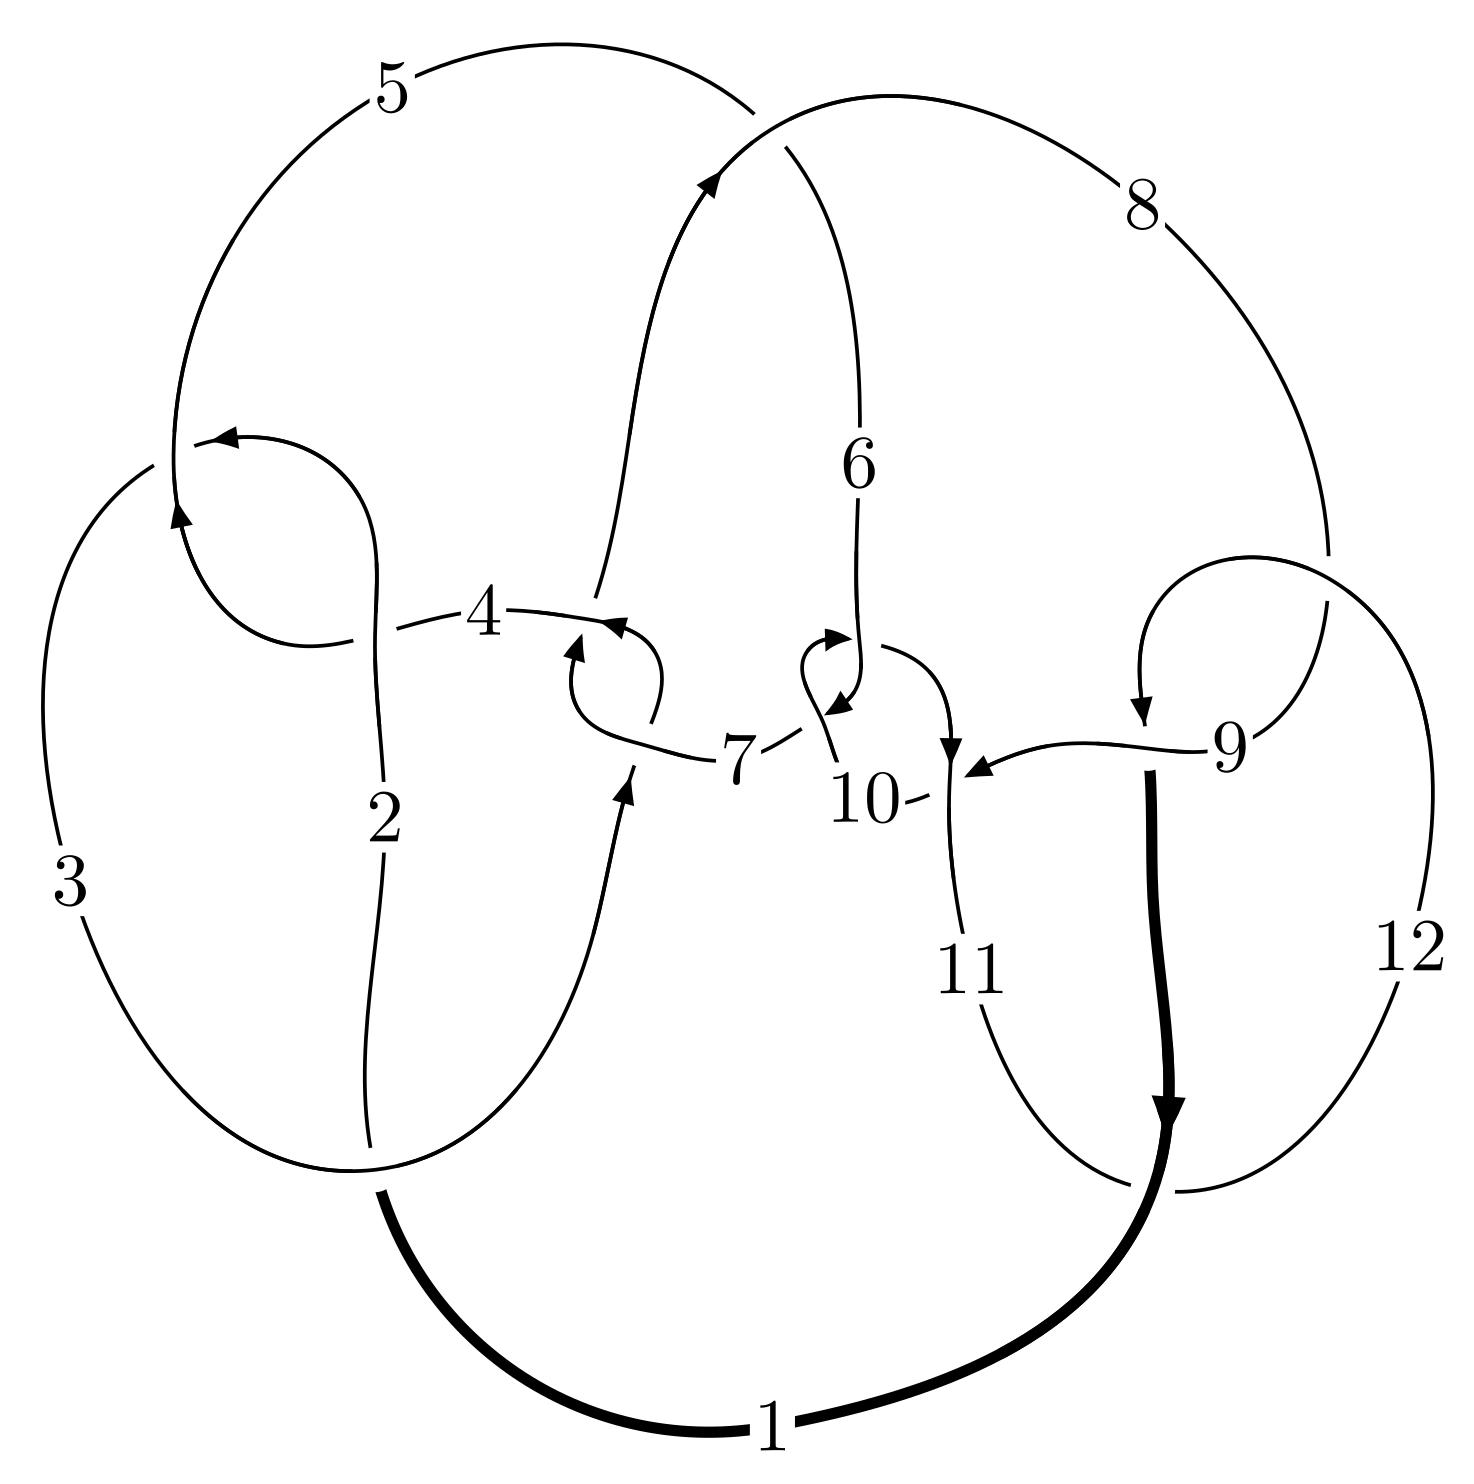
\includegraphics[width=112pt]{../../../GIT/diagram.site/Diagrams/png/841_12a_0040.png}\\
\ \ \ A knot diagram\footnotemark}&
\allowdisplaybreaks
\textbf{Linearized knot diagam} \\
\cline{2-2}
 &
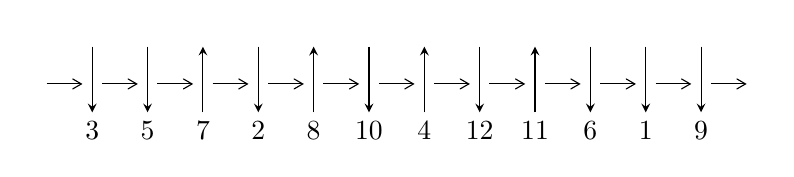
\begin{tikzpicture}[x=20pt, y=17pt]
	% nodes
	\node (C0) at (0, 0) {};
	\node (C1) at (1, 0) {};
	\node (C1U) at (1, +1) {};
	\node (C1D) at (1, -1) {3};

	\node (C2) at (2, 0) {};
	\node (C2U) at (2, +1) {};
	\node (C2D) at (2, -1) {5};

	\node (C3) at (3, 0) {};
	\node (C3U) at (3, +1) {};
	\node (C3D) at (3, -1) {7};

	\node (C4) at (4, 0) {};
	\node (C4U) at (4, +1) {};
	\node (C4D) at (4, -1) {2};

	\node (C5) at (5, 0) {};
	\node (C5U) at (5, +1) {};
	\node (C5D) at (5, -1) {8};

	\node (C6) at (6, 0) {};
	\node (C6U) at (6, +1) {};
	\node (C6D) at (6, -1) {10};

	\node (C7) at (7, 0) {};
	\node (C7U) at (7, +1) {};
	\node (C7D) at (7, -1) {4};

	\node (C8) at (8, 0) {};
	\node (C8U) at (8, +1) {};
	\node (C8D) at (8, -1) {12};

	\node (C9) at (9, 0) {};
	\node (C9U) at (9, +1) {};
	\node (C9D) at (9, -1) {11};

	\node (C10) at (10, 0) {};
	\node (C10U) at (10, +1) {};
	\node (C10D) at (10, -1) {6};

	\node (C11) at (11, 0) {};
	\node (C11U) at (11, +1) {};
	\node (C11D) at (11, -1) {1};

	\node (C12) at (12, 0) {};
	\node (C12U) at (12, +1) {};
	\node (C12D) at (12, -1) {9};
	\node (C13) at (13, 0) {};

	% arrows
	\draw[->,>={angle 60}]
	(C0) edge (C1) (C1) edge (C2) (C2) edge (C3) (C3) edge (C4) (C4) edge (C5) (C5) edge (C6) (C6) edge (C7) (C7) edge (C8) (C8) edge (C9) (C9) edge (C10) (C10) edge (C11) (C11) edge (C12) (C12) edge (C13) ;	\draw[->,>=stealth]
	(C1U) edge (C1D) (C2U) edge (C2D) (C3D) edge (C3U) (C4U) edge (C4D) (C5D) edge (C5U) (C6U) edge (C6D) (C7D) edge (C7U) (C8U) edge (C8D) (C9D) edge (C9U) (C10U) edge (C10D) (C11U) edge (C11D) (C12U) edge (C12D) ;
	\end{tikzpicture} \\
\hhline{~~} \\& 
\textbf{Solving Sequence} \\ \cline{2-2} 
 &
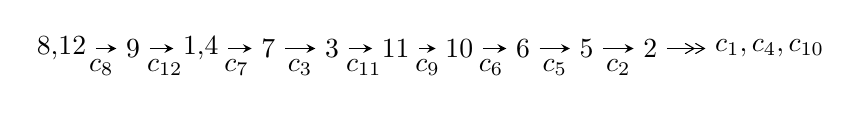
\begin{tikzpicture}[x=23pt, y=7pt]
	% node
	\node (A0) at (-1/8, 0) {8,12};
	\node (A1) at (1, 0) {9};
	\node (A2) at (33/16, 0) {1,4};
	\node (A3) at (25/8, 0) {7};
	\node (A4) at (33/8, 0) {3};
	\node (A5) at (41/8, 0) {11};
	\node (A6) at (49/8, 0) {10};
	\node (A7) at (57/8, 0) {6};
	\node (A8) at (65/8, 0) {5};
	\node (A9) at (73/8, 0) {2};
	\node (C1) at (1/2, -1) {$c_{8}$};
	\node (C2) at (3/2, -1) {$c_{12}$};
	\node (C3) at (21/8, -1) {$c_{7}$};
	\node (C4) at (29/8, -1) {$c_{3}$};
	\node (C5) at (37/8, -1) {$c_{11}$};
	\node (C6) at (45/8, -1) {$c_{9}$};
	\node (C7) at (53/8, -1) {$c_{6}$};
	\node (C8) at (61/8, -1) {$c_{5}$};
	\node (C9) at (69/8, -1) {$c_{2}$};
	\node (A10) at (11, 0) {$c_{1},c_{4},c_{10}$};

	% edge
	\draw[->,>=stealth]	
	(A0) edge (A1) (A1) edge (A2) (A2) edge (A3) (A3) edge (A4) (A4) edge (A5) (A5) edge (A6) (A6) edge (A7) (A7) edge (A8) (A8) edge (A9) ;
	\draw[->>,>={angle 60}]	
	(A9) edge (A10);
\end{tikzpicture} \\ 

\end{tabular} \\

\footnotetext{
The image of knot diagram is generated by the software ``\textbf{Draw programme}" developed by Andrew Bartholomew(\url{http://www.layer8.co.uk/maths/draw/index.htm\#Running-draw}), where we modified some parts for our purpose(\url{https://github.com/CATsTAILs/LinksPainter}).
}\phantom \\ \newline 
\centering \textbf{Ideals for irreducible components\footnotemark of $X_{\text{par}}$} 
 
\begin{align*}
I^u_{1}&=\langle 
2.52476\times10^{40} u^{119}+1.85032\times10^{41} u^{118}+\cdots+3.97571\times10^{38} b+3.69260\times10^{40},\\
\phantom{I^u_{1}}&\phantom{= \langle  }1.98154\times10^{40} u^{119}+1.49672\times10^{41} u^{118}+\cdots+1.98786\times10^{38} a+3.56279\times10^{40},\;u^{120}+8 u^{119}+\cdots+8 u+1\rangle \\
I^u_{2}&=\langle 
b,\;u^8+2 u^7- u^6-4 u^5- u^4+3 u^3+3 u^2+a+2 u,\;u^9+u^8-2 u^7-3 u^6+u^5+3 u^4+2 u^3- u-1\rangle \\
I^u_{3}&=\langle 
2 a^5-2 a^4+7 a^3-5 a^2+3 b+a-4,\;a^6+4 a^4+a^3+4 a^2+1,\;u-1\rangle \\
\\
\end{align*}
\raggedright * 3 irreducible components of $\dim_{\mathbb{C}}=0$, with total 135 representations.\\
\footnotetext{All coefficients of polynomials are rational numbers. But the coefficients are sometimes approximated in decimal forms when there is not enough margin.}
\newpage
\renewcommand{\arraystretch}{1}
\centering \section*{I. $I^u_{1}= \langle 2.52\times10^{40} u^{119}+1.85\times10^{41} u^{118}+\cdots+3.98\times10^{38} b+3.69\times10^{40},\;1.98\times10^{40} u^{119}+1.50\times10^{41} u^{118}+\cdots+1.99\times10^{38} a+3.56\times10^{40},\;u^{120}+8 u^{119}+\cdots+8 u+1 \rangle$}
\flushleft \textbf{(i) Arc colorings}\\
\begin{tabular}{m{7pt} m{180pt} m{7pt} m{180pt} }
\flushright $a_{8}=$&$\begin{pmatrix}1\\0\end{pmatrix}$ \\
\flushright $a_{12}=$&$\begin{pmatrix}0\\u\end{pmatrix}$ \\
\flushright $a_{9}=$&$\begin{pmatrix}1\\u^2\end{pmatrix}$ \\
\flushright $a_{1}=$&$\begin{pmatrix}- u\\- u^3+u\end{pmatrix}$ \\
\flushright $a_{4}=$&$\begin{pmatrix}-99.6821 u^{119}-752.933 u^{118}+\cdots-1132.22 u-179.228\\-63.5047 u^{119}-465.406 u^{118}+\cdots-610.082 u-92.8790\end{pmatrix}$ \\
\flushright $a_{7}=$&$\begin{pmatrix}-87.8357 u^{119}-646.404 u^{118}+\cdots-906.733 u-143.815\\-72.6685 u^{119}-538.693 u^{118}+\cdots-759.203 u-119.616\end{pmatrix}$ \\
\flushright $a_{3}=$&$\begin{pmatrix}-58.4140 u^{119}-454.008 u^{118}+\cdots-741.967 u-116.664\\-11.7388 u^{119}-99.1517 u^{118}+\cdots-221.718 u-34.2318\end{pmatrix}$ \\
\flushright $a_{11}=$&$\begin{pmatrix}u^3\\u^5- u^3+u\end{pmatrix}$ \\
\flushright $a_{10}=$&$\begin{pmatrix}u^6- u^4+1\\u^8-2 u^6+2 u^4\end{pmatrix}$ \\
\flushright $a_{6}=$&$\begin{pmatrix}-142.741 u^{119}-1051.82 u^{118}+\cdots-1483.16 u-234.293\\-79.4077 u^{119}-581.716 u^{118}+\cdots-788.076 u-124.403\end{pmatrix}$ \\
\flushright $a_{5}=$&$\begin{pmatrix}-63.3338 u^{119}-470.103 u^{118}+\cdots-695.081 u-109.889\\-79.4077 u^{119}-581.716 u^{118}+\cdots-788.076 u-124.403\end{pmatrix}$ \\
\flushright $a_{2}=$&$\begin{pmatrix}-101.184 u^{119}-771.740 u^{118}+\cdots-1234.87 u-197.448\\-73.1735 u^{119}-538.032 u^{118}+\cdots-737.816 u-115.113\end{pmatrix}$\\&\end{tabular}
\flushleft \textbf{(ii) Obstruction class $= -1$}\\~\\
\flushleft \textbf{(iii) Cusp Shapes $= 155.044 u^{119}+1104.19 u^{118}+\cdots+1214.15 u+168.050$}\\~\\
\newpage\renewcommand{\arraystretch}{1}
\flushleft \textbf{(iv) u-Polynomials at the component}\newline \\
\begin{tabular}{m{50pt}|m{274pt}}
Crossings & \hspace{64pt}u-Polynomials at each crossing \\
\hline $$\begin{aligned}c_{1}\end{aligned}$$&$\begin{aligned}
&u^{120}+57 u^{119}+\cdots+451 u+1
\end{aligned}$\\
\hline $$\begin{aligned}c_{2},c_{4}\end{aligned}$$&$\begin{aligned}
&u^{120}-11 u^{119}+\cdots+27 u-1
\end{aligned}$\\
\hline $$\begin{aligned}c_{3},c_{7}\end{aligned}$$&$\begin{aligned}
&u^{120}-2 u^{119}+\cdots-512 u+512
\end{aligned}$\\
\hline $$\begin{aligned}c_{5}\end{aligned}$$&$\begin{aligned}
&u^{120}+3 u^{119}+\cdots-3758933 u-444601
\end{aligned}$\\
\hline $$\begin{aligned}c_{6},c_{10}\end{aligned}$$&$\begin{aligned}
&u^{120}+2 u^{119}+\cdots-128 u-64
\end{aligned}$\\
\hline $$\begin{aligned}c_{8},c_{12}\end{aligned}$$&$\begin{aligned}
&u^{120}-8 u^{119}+\cdots-8 u+1
\end{aligned}$\\
\hline $$\begin{aligned}c_{9}\end{aligned}$$&$\begin{aligned}
&u^{120}-42 u^{119}+\cdots-106496 u+4096
\end{aligned}$\\
\hline $$\begin{aligned}c_{11}\end{aligned}$$&$\begin{aligned}
&u^{120}+64 u^{119}+\cdots+8 u+1
\end{aligned}$\\
\hline
\end{tabular}\\~\\
\newpage\renewcommand{\arraystretch}{1}
\flushleft \textbf{(v) Riley Polynomials at the component}\newline \\
\begin{tabular}{m{50pt}|m{274pt}}
Crossings & \hspace{64pt}Riley Polynomials at each crossing \\
\hline $$\begin{aligned}c_{1}\end{aligned}$$&$\begin{aligned}
&y^{120}+23 y^{119}+\cdots-187035 y+1
\end{aligned}$\\
\hline $$\begin{aligned}c_{2},c_{4}\end{aligned}$$&$\begin{aligned}
&y^{120}-57 y^{119}+\cdots-451 y+1
\end{aligned}$\\
\hline $$\begin{aligned}c_{3},c_{7}\end{aligned}$$&$\begin{aligned}
&y^{120}-60 y^{119}+\cdots-11796480 y+262144
\end{aligned}$\\
\hline $$\begin{aligned}c_{5}\end{aligned}$$&$\begin{aligned}
&y^{120}-21 y^{119}+\cdots-9546190035499 y+197670049201
\end{aligned}$\\
\hline $$\begin{aligned}c_{6},c_{10}\end{aligned}$$&$\begin{aligned}
&y^{120}+42 y^{119}+\cdots+106496 y+4096
\end{aligned}$\\
\hline $$\begin{aligned}c_{8},c_{12}\end{aligned}$$&$\begin{aligned}
&y^{120}-64 y^{119}+\cdots-8 y+1
\end{aligned}$\\
\hline $$\begin{aligned}c_{9}\end{aligned}$$&$\begin{aligned}
&y^{120}+62 y^{119}+\cdots-511705088 y+16777216
\end{aligned}$\\
\hline $$\begin{aligned}c_{11}\end{aligned}$$&$\begin{aligned}
&y^{120}-8 y^{119}+\cdots-64 y+1
\end{aligned}$\\
\hline
\end{tabular}\\~\\
\newpage\flushleft \textbf{(vi) Complex Volumes and Cusp Shapes}
$$\begin{array}{c|c|c}  
\text{Solutions to }I^u_{1}& \I (\text{vol} + \sqrt{-1}CS) & \text{Cusp shape}\\
 \hline 
\begin{aligned}
u &= -0.781703 + 0.626996 I \\
a &= \phantom{-}2.53481 - 0.75078 I \\
b &= -0.897256 - 0.066842 I\end{aligned}
 & \phantom{-}1.45619 + 2.43204 I & \phantom{-0.000000 } 0 \\ \hline\begin{aligned}
u &= -0.781703 - 0.626996 I \\
a &= \phantom{-}2.53481 + 0.75078 I \\
b &= -0.897256 + 0.066842 I\end{aligned}
 & \phantom{-}1.45619 - 2.43204 I & \phantom{-0.000000 } 0 \\ \hline\begin{aligned}
u &= -0.688922 + 0.732659 I \\
a &= \phantom{-}1.61210 - 0.53654 I \\
b &= -1.277420 + 0.530341 I\end{aligned}
 & \phantom{-}6.62514 - 5.23780 I & \phantom{-0.000000 } 0 \\ \hline\begin{aligned}
u &= -0.688922 - 0.732659 I \\
a &= \phantom{-}1.61210 + 0.53654 I \\
b &= -1.277420 - 0.530341 I\end{aligned}
 & \phantom{-}6.62514 + 5.23780 I & \phantom{-0.000000 } 0 \\ \hline\begin{aligned}
u &= -0.739899 + 0.655965 I \\
a &= \phantom{-}0.767226 + 0.255470 I \\
b &= -0.164900 - 1.010320 I\end{aligned}
 & \phantom{-}3.04826 + 0.29752 I & \phantom{-0.000000 } 0 \\ \hline\begin{aligned}
u &= -0.739899 - 0.655965 I \\
a &= \phantom{-}0.767226 - 0.255470 I \\
b &= -0.164900 + 1.010320 I\end{aligned}
 & \phantom{-}3.04826 - 0.29752 I & \phantom{-0.000000 } 0 \\ \hline\begin{aligned}
u &= -0.733582 + 0.717890 I \\
a &= -1.83320 + 0.64066 I \\
b &= \phantom{-}1.305000 - 0.285363 I\end{aligned}
 & \phantom{-}8.21310 + 0.50687 I & \phantom{-0.000000 } 0 \\ \hline\begin{aligned}
u &= -0.733582 - 0.717890 I \\
a &= -1.83320 - 0.64066 I \\
b &= \phantom{-}1.305000 + 0.285363 I\end{aligned}
 & \phantom{-}8.21310 - 0.50687 I & \phantom{-0.000000 } 0 \\ \hline\begin{aligned}
u &= \phantom{-}0.930786 + 0.465334 I \\
a &= -1.02154 - 1.67472 I \\
b &= \phantom{-}1.180540 + 0.406202 I\end{aligned}
 & \phantom{-}0.64675 + 2.54597 I & \phantom{-0.000000 } 0 \\ \hline\begin{aligned}
u &= \phantom{-}0.930786 - 0.465334 I \\
a &= -1.02154 + 1.67472 I \\
b &= \phantom{-}1.180540 - 0.406202 I\end{aligned}
 & \phantom{-}0.64675 - 2.54597 I & \phantom{-0.000000 } 0\\
 \hline 
 \end{array}$$\newpage$$\begin{array}{c|c|c}  
\text{Solutions to }I^u_{1}& \I (\text{vol} + \sqrt{-1}CS) & \text{Cusp shape}\\
 \hline 
\begin{aligned}
u &= -0.819870 + 0.648210 I \\
a &= -0.568752 - 0.480301 I \\
b &= -0.257485 + 1.034380 I\end{aligned}
 & \phantom{-}2.81901 + 4.71117 I & \phantom{-0.000000 } 0 \\ \hline\begin{aligned}
u &= -0.819870 - 0.648210 I \\
a &= -0.568752 + 0.480301 I \\
b &= -0.257485 - 1.034380 I\end{aligned}
 & \phantom{-}2.81901 - 4.71117 I & \phantom{-0.000000 } 0 \\ \hline\begin{aligned}
u &= \phantom{-}1.072720 + 0.077721 I \\
a &= -0.20436 - 2.27899 I \\
b &= -0.211326 - 0.578062 I\end{aligned}
 & -3.19317 - 0.58424 I & \phantom{-0.000000 } 0 \\ \hline\begin{aligned}
u &= \phantom{-}1.072720 - 0.077721 I \\
a &= -0.20436 + 2.27899 I \\
b &= -0.211326 + 0.578062 I\end{aligned}
 & -3.19317 + 0.58424 I & \phantom{-0.000000 } 0 \\ \hline\begin{aligned}
u &= -0.226064 + 0.885039 I \\
a &= \phantom{-}1.57130 + 0.52144 I \\
b &= -1.221930 + 0.677956 I\end{aligned}
 & \phantom{-}2.10205 - 12.84790 I & \phantom{-0.000000 } 0 \\ \hline\begin{aligned}
u &= -0.226064 - 0.885039 I \\
a &= \phantom{-}1.57130 - 0.52144 I \\
b &= -1.221930 - 0.677956 I\end{aligned}
 & \phantom{-}2.10205 + 12.84790 I & \phantom{-0.000000 } 0 \\ \hline\begin{aligned}
u &= -0.841471 + 0.691793 I \\
a &= -2.07690 + 1.04697 I \\
b &= \phantom{-}1.296310 + 0.355054 I\end{aligned}
 & \phantom{-}7.89915 + 4.80277 I & \phantom{-0.000000 } 0 \\ \hline\begin{aligned}
u &= -0.841471 - 0.691793 I \\
a &= -2.07690 - 1.04697 I \\
b &= \phantom{-}1.296310 - 0.355054 I\end{aligned}
 & \phantom{-}7.89915 - 4.80277 I & \phantom{-0.000000 } 0 \\ \hline\begin{aligned}
u &= -0.248169 + 0.867541 I \\
a &= -1.72098 - 0.45454 I \\
b &= \phantom{-}1.237400 - 0.490795 I\end{aligned}
 & \phantom{-}4.40266 - 7.18738 I & \phantom{-0.000000 } 0 \\ \hline\begin{aligned}
u &= -0.248169 - 0.867541 I \\
a &= -1.72098 + 0.45454 I \\
b &= \phantom{-}1.237400 + 0.490795 I\end{aligned}
 & \phantom{-}4.40266 + 7.18738 I & \phantom{-0.000000 } 0\\
 \hline 
 \end{array}$$\newpage$$\begin{array}{c|c|c}  
\text{Solutions to }I^u_{1}& \I (\text{vol} + \sqrt{-1}CS) & \text{Cusp shape}\\
 \hline 
\begin{aligned}
u &= -0.798069 + 0.417778 I \\
a &= -0.028492 - 0.471920 I \\
b &= -0.661694 - 0.043069 I\end{aligned}
 & \phantom{-}1.21358 + 1.83340 I & \phantom{-0.000000 } 0 \\ \hline\begin{aligned}
u &= -0.798069 - 0.417778 I \\
a &= -0.028492 + 0.471920 I \\
b &= -0.661694 + 0.043069 I\end{aligned}
 & \phantom{-}1.21358 - 1.83340 I & \phantom{-0.000000 } 0 \\ \hline\begin{aligned}
u &= \phantom{-}1.004720 + 0.468278 I \\
a &= \phantom{-}1.28653 + 1.75341 I \\
b &= -1.221750 - 0.109820 I\end{aligned}
 & \phantom{-}1.69311 - 2.74237 I & \phantom{-0.000000 } 0 \\ \hline\begin{aligned}
u &= \phantom{-}1.004720 - 0.468278 I \\
a &= \phantom{-}1.28653 - 1.75341 I \\
b &= -1.221750 + 0.109820 I\end{aligned}
 & \phantom{-}1.69311 + 2.74237 I & \phantom{-0.000000 } 0 \\ \hline\begin{aligned}
u &= -0.878883 + 0.685866 I \\
a &= \phantom{-}2.04246 - 1.14516 I \\
b &= -1.272340 - 0.584117 I\end{aligned}
 & \phantom{-}6.07322 + 10.56780 I & \phantom{-0.000000 } 0 \\ \hline\begin{aligned}
u &= -0.878883 - 0.685866 I \\
a &= \phantom{-}2.04246 + 1.14516 I \\
b &= -1.272340 + 0.584117 I\end{aligned}
 & \phantom{-}6.07322 - 10.56780 I & \phantom{-0.000000 } 0 \\ \hline\begin{aligned}
u &= -0.344653 + 0.812462 I \\
a &= -1.85816 - 0.05813 I \\
b &= \phantom{-}1.296950 + 0.114963 I\end{aligned}
 & \phantom{-}6.09868 - 3.26636 I & \phantom{-0.000000 } 0 \\ \hline\begin{aligned}
u &= -0.344653 - 0.812462 I \\
a &= -1.85816 + 0.05813 I \\
b &= \phantom{-}1.296950 - 0.114963 I\end{aligned}
 & \phantom{-}6.09868 + 3.26636 I & \phantom{-0.000000 } 0 \\ \hline\begin{aligned}
u &= -0.401546 + 0.783989 I \\
a &= \phantom{-}1.75354 - 0.06110 I \\
b &= -1.259800 - 0.384650 I\end{aligned}
 & \phantom{-}5.11752 + 2.33858 I & \phantom{-0.000000 } 0 \\ \hline\begin{aligned}
u &= -0.401546 - 0.783989 I \\
a &= \phantom{-}1.75354 + 0.06110 I \\
b &= -1.259800 + 0.384650 I\end{aligned}
 & \phantom{-}5.11752 - 2.33858 I & \phantom{-0.000000 } 0\\
 \hline 
 \end{array}$$\newpage$$\begin{array}{c|c|c}  
\text{Solutions to }I^u_{1}& \I (\text{vol} + \sqrt{-1}CS) & \text{Cusp shape}\\
 \hline 
\begin{aligned}
u &= -0.233066 + 0.838650 I \\
a &= \phantom{-}0.082248 + 0.246084 I \\
b &= -0.431383 - 1.042700 I\end{aligned}
 & -0.41671 - 6.60155 I & \phantom{-0.000000 } 0 \\ \hline\begin{aligned}
u &= -0.233066 - 0.838650 I \\
a &= \phantom{-}0.082248 - 0.246084 I \\
b &= -0.431383 + 1.042700 I\end{aligned}
 & -0.41671 + 6.60155 I & \phantom{-0.000000 } 0 \\ \hline\begin{aligned}
u &= \phantom{-}0.863965\phantom{ +0.000000I} \\
a &= -0.644795\phantom{ +0.000000I} \\
b &= \phantom{-}0.219021\phantom{ +0.000000I}\end{aligned}
 & -1.25564\phantom{ +0.000000I} & \phantom{-0.000000 } 0 \\ \hline\begin{aligned}
u &= -1.082180 + 0.408010 I \\
a &= -0.060771 + 0.358868 I \\
b &= -1.056880 + 0.541010 I\end{aligned}
 & -0.617111 + 1.136830 I & \phantom{-0.000000 } 0 \\ \hline\begin{aligned}
u &= -1.082180 - 0.408010 I \\
a &= -0.060771 - 0.358868 I \\
b &= -1.056880 - 0.541010 I\end{aligned}
 & -0.617111 - 1.136830 I & \phantom{-0.000000 } 0 \\ \hline\begin{aligned}
u &= -0.228884 + 0.809806 I \\
a &= \phantom{-}2.14403 + 0.63084 I \\
b &= -0.913467 + 0.317981 I\end{aligned}
 & -1.37934 - 4.06817 I & \phantom{-0.000000 } 0 \\ \hline\begin{aligned}
u &= -0.228884 - 0.809806 I \\
a &= \phantom{-}2.14403 - 0.63084 I \\
b &= -0.913467 - 0.317981 I\end{aligned}
 & -1.37934 + 4.06817 I & \phantom{-0.000000 } 0 \\ \hline\begin{aligned}
u &= \phantom{-}1.091890 + 0.407398 I \\
a &= -1.225800 - 0.382164 I \\
b &= -0.106806 - 0.841935 I\end{aligned}
 & -3.25950 - 1.43414 I & \phantom{-0.000000 } 0 \\ \hline\begin{aligned}
u &= \phantom{-}1.091890 - 0.407398 I \\
a &= -1.225800 + 0.382164 I \\
b &= -0.106806 + 0.841935 I\end{aligned}
 & -3.25950 + 1.43414 I & \phantom{-0.000000 } 0 \\ \hline\begin{aligned}
u &= -1.114220 + 0.383038 I \\
a &= \phantom{-}0.298421 - 0.602605 I \\
b &= \phantom{-}1.117930 - 0.678993 I\end{aligned}
 & -3.13753 - 4.01738 I & \phantom{-0.000000 } 0\\
 \hline 
 \end{array}$$\newpage$$\begin{array}{c|c|c}  
\text{Solutions to }I^u_{1}& \I (\text{vol} + \sqrt{-1}CS) & \text{Cusp shape}\\
 \hline 
\begin{aligned}
u &= -1.114220 - 0.383038 I \\
a &= \phantom{-}0.298421 + 0.602605 I \\
b &= \phantom{-}1.117930 + 0.678993 I\end{aligned}
 & -3.13753 + 4.01738 I & \phantom{-0.000000 } 0 \\ \hline\begin{aligned}
u &= -0.114192 + 0.811962 I \\
a &= \phantom{-}0.195578 + 0.002860 I \\
b &= -0.774547 - 0.295093 I\end{aligned}
 & -1.84565 - 1.28021 I & \phantom{-0.000000 } 0 \\ \hline\begin{aligned}
u &= -0.114192 - 0.811962 I \\
a &= \phantom{-}0.195578 - 0.002860 I \\
b &= -0.774547 + 0.295093 I\end{aligned}
 & -1.84565 + 1.28021 I & \phantom{-0.000000 } 0 \\ \hline\begin{aligned}
u &= -0.263583 + 0.772995 I \\
a &= \phantom{-}0.048817 - 0.164759 I \\
b &= \phantom{-}0.062093 + 0.937483 I\end{aligned}
 & \phantom{-}0.77417 - 2.19825 I & \phantom{-0.000000 } 0 \\ \hline\begin{aligned}
u &= -0.263583 - 0.772995 I \\
a &= \phantom{-}0.048817 + 0.164759 I \\
b &= \phantom{-}0.062093 - 0.937483 I\end{aligned}
 & \phantom{-}0.77417 + 2.19825 I & \phantom{-0.000000 } 0 \\ \hline\begin{aligned}
u &= \phantom{-}1.145450 + 0.314699 I \\
a &= -0.630962 - 1.037490 I \\
b &= \phantom{-}0.172083 - 0.746812 I\end{aligned}
 & -3.47727 - 0.99083 I & \phantom{-0.000000 } 0 \\ \hline\begin{aligned}
u &= \phantom{-}1.145450 - 0.314699 I \\
a &= -0.630962 + 1.037490 I \\
b &= \phantom{-}0.172083 + 0.746812 I\end{aligned}
 & -3.47727 + 0.99083 I & \phantom{-0.000000 } 0 \\ \hline\begin{aligned}
u &= -1.108160 + 0.433990 I \\
a &= -0.355791 + 1.337260 I \\
b &= \phantom{-}0.570690 + 0.939425 I\end{aligned}
 & -4.90498 + 1.93971 I & \phantom{-0.000000 } 0 \\ \hline\begin{aligned}
u &= -1.108160 - 0.433990 I \\
a &= -0.355791 - 1.337260 I \\
b &= \phantom{-}0.570690 - 0.939425 I\end{aligned}
 & -4.90498 - 1.93971 I & \phantom{-0.000000 } 0 \\ \hline\begin{aligned}
u &= \phantom{-}1.118830 + 0.445202 I \\
a &= -1.95584 - 2.05447 I \\
b &= \phantom{-}0.869061 - 0.363739 I\end{aligned}
 & -5.50041 - 3.10765 I & \phantom{-0.000000 } 0\\
 \hline 
 \end{array}$$\newpage$$\begin{array}{c|c|c}  
\text{Solutions to }I^u_{1}& \I (\text{vol} + \sqrt{-1}CS) & \text{Cusp shape}\\
 \hline 
\begin{aligned}
u &= \phantom{-}1.118830 - 0.445202 I \\
a &= -1.95584 + 2.05447 I \\
b &= \phantom{-}0.869061 + 0.363739 I\end{aligned}
 & -5.50041 + 3.10765 I & \phantom{-0.000000 } 0 \\ \hline\begin{aligned}
u &= -1.119840 + 0.453707 I \\
a &= -0.521942 - 0.703698 I \\
b &= \phantom{-}0.849724 - 0.535024 I\end{aligned}
 & -5.43931 + 4.53491 I & \phantom{-0.000000 } 0 \\ \hline\begin{aligned}
u &= -1.119840 - 0.453707 I \\
a &= -0.521942 + 0.703698 I \\
b &= \phantom{-}0.849724 + 0.535024 I\end{aligned}
 & -5.43931 - 4.53491 I & \phantom{-0.000000 } 0 \\ \hline\begin{aligned}
u &= -0.777873 + 0.136267 I \\
a &= \phantom{-}0.441442 + 1.221480 I \\
b &= \phantom{-}1.019780 + 0.579374 I\end{aligned}
 & -1.06043 + 6.07967 I & \phantom{-0.000000 } 0 \\ \hline\begin{aligned}
u &= -0.777873 - 0.136267 I \\
a &= \phantom{-}0.441442 - 1.221480 I \\
b &= \phantom{-}1.019780 - 0.579374 I\end{aligned}
 & -1.06043 - 6.07967 I & \phantom{-0.000000 } 0 \\ \hline\begin{aligned}
u &= \phantom{-}1.116780 + 0.468489 I \\
a &= \phantom{-}1.380320 - 0.108317 I \\
b &= \phantom{-}0.451699 + 1.005900 I\end{aligned}
 & -4.64482 - 5.60149 I & \phantom{-0.000000 } 0 \\ \hline\begin{aligned}
u &= \phantom{-}1.116780 - 0.468489 I \\
a &= \phantom{-}1.380320 + 0.108317 I \\
b &= \phantom{-}0.451699 - 1.005900 I\end{aligned}
 & -4.64482 + 5.60149 I & \phantom{-0.000000 } 0 \\ \hline\begin{aligned}
u &= \phantom{-}0.617737 + 0.488236 I \\
a &= -2.91600 - 0.23481 I \\
b &= \phantom{-}1.193780 - 0.512097 I\end{aligned}
 & \phantom{-}1.56344 - 6.54073 I & \phantom{-0.000000 } 0 \\ \hline\begin{aligned}
u &= \phantom{-}0.617737 - 0.488236 I \\
a &= -2.91600 + 0.23481 I \\
b &= \phantom{-}1.193780 + 0.512097 I\end{aligned}
 & \phantom{-}1.56344 + 6.54073 I & \phantom{-0.000000 } 0 \\ \hline\begin{aligned}
u &= \phantom{-}1.108140 + 0.494518 I \\
a &= \phantom{-}1.60623 + 2.13884 I \\
b &= -1.200220 + 0.485456 I\end{aligned}
 & \phantom{-}0.04434 - 6.17641 I & \phantom{-0.000000 } 0\\
 \hline 
 \end{array}$$\newpage$$\begin{array}{c|c|c}  
\text{Solutions to }I^u_{1}& \I (\text{vol} + \sqrt{-1}CS) & \text{Cusp shape}\\
 \hline 
\begin{aligned}
u &= \phantom{-}1.108140 - 0.494518 I \\
a &= \phantom{-}1.60623 - 2.13884 I \\
b &= -1.200220 - 0.485456 I\end{aligned}
 & \phantom{-}0.04434 + 6.17641 I & \phantom{-0.000000 } 0 \\ \hline\begin{aligned}
u &= -1.121190 + 0.486520 I \\
a &= \phantom{-}0.532816 - 0.923881 I \\
b &= -0.373734 - 0.813785 I\end{aligned}
 & -2.64934 + 6.07508 I & \phantom{-0.000000 } 0 \\ \hline\begin{aligned}
u &= -1.121190 - 0.486520 I \\
a &= \phantom{-}0.532816 + 0.923881 I \\
b &= -0.373734 + 0.813785 I\end{aligned}
 & -2.64934 - 6.07508 I & \phantom{-0.000000 } 0 \\ \hline\begin{aligned}
u &= \phantom{-}1.224670 + 0.160747 I \\
a &= -0.065857 - 0.607777 I \\
b &= \phantom{-}1.163270 - 0.153221 I\end{aligned}
 & \phantom{-}0.928537 + 0.392500 I & \phantom{-0.000000 } 0 \\ \hline\begin{aligned}
u &= \phantom{-}1.224670 - 0.160747 I \\
a &= -0.065857 + 0.607777 I \\
b &= \phantom{-}1.163270 + 0.153221 I\end{aligned}
 & \phantom{-}0.928537 - 0.392500 I & \phantom{-0.000000 } 0 \\ \hline\begin{aligned}
u &= -1.090900 + 0.581156 I \\
a &= \phantom{-}0.667582 - 0.986969 I \\
b &= -1.279380 + 0.305378 I\end{aligned}
 & \phantom{-}3.07488 + 2.77369 I & \phantom{-0.000000 } 0 \\ \hline\begin{aligned}
u &= -1.090900 - 0.581156 I \\
a &= \phantom{-}0.667582 + 0.986969 I \\
b &= -1.279380 - 0.305378 I\end{aligned}
 & \phantom{-}3.07488 - 2.77369 I & \phantom{-0.000000 } 0 \\ \hline\begin{aligned}
u &= \phantom{-}1.130050 + 0.504249 I \\
a &= -1.59951 - 2.24133 I \\
b &= \phantom{-}1.200410 - 0.671678 I\end{aligned}
 & -2.26176 - 11.72400 I & \phantom{-0.000000 } 0 \\ \hline\begin{aligned}
u &= \phantom{-}1.130050 - 0.504249 I \\
a &= -1.59951 + 2.24133 I \\
b &= \phantom{-}1.200410 + 0.671678 I\end{aligned}
 & -2.26176 + 11.72400 I & \phantom{-0.000000 } 0 \\ \hline\begin{aligned}
u &= \phantom{-}1.240540 + 0.097824 I \\
a &= -0.114954 + 0.943587 I \\
b &= -1.158460 + 0.463847 I\end{aligned}
 & -0.36881 - 4.75701 I & \phantom{-0.000000 } 0\\
 \hline 
 \end{array}$$\newpage$$\begin{array}{c|c|c}  
\text{Solutions to }I^u_{1}& \I (\text{vol} + \sqrt{-1}CS) & \text{Cusp shape}\\
 \hline 
\begin{aligned}
u &= \phantom{-}1.240540 - 0.097824 I \\
a &= -0.114954 - 0.943587 I \\
b &= -1.158460 - 0.463847 I\end{aligned}
 & -0.36881 + 4.75701 I & \phantom{-0.000000 } 0 \\ \hline\begin{aligned}
u &= \phantom{-}1.205540 + 0.311353 I \\
a &= \phantom{-}0.787036 - 0.684011 I \\
b &= -0.825731 - 0.396066 I\end{aligned}
 & -5.80900 + 0.49213 I & \phantom{-0.000000 } 0 \\ \hline\begin{aligned}
u &= \phantom{-}1.205540 - 0.311353 I \\
a &= \phantom{-}0.787036 + 0.684011 I \\
b &= -0.825731 + 0.396066 I\end{aligned}
 & -5.80900 - 0.49213 I & \phantom{-0.000000 } 0 \\ \hline\begin{aligned}
u &= -0.014569 + 0.745385 I \\
a &= -0.132373 + 0.263093 I \\
b &= \phantom{-}0.852646 - 0.399361 I\end{aligned}
 & -2.28381 - 4.26886 I & -4.00000 + 7.23139 I \\ \hline\begin{aligned}
u &= -0.014569 - 0.745385 I \\
a &= -0.132373 - 0.263093 I \\
b &= \phantom{-}0.852646 + 0.399361 I\end{aligned}
 & -2.28381 + 4.26886 I & -4.00000 - 7.23139 I \\ \hline\begin{aligned}
u &= -0.676491 + 0.294104 I \\
a &= \phantom{-}0.092796 - 0.977502 I \\
b &= -0.769091 - 0.387965 I\end{aligned}
 & \phantom{-}1.10898 + 1.72747 I & \phantom{-}2.65279 - 4.70086 I \\ \hline\begin{aligned}
u &= -0.676491 - 0.294104 I \\
a &= \phantom{-}0.092796 + 0.977502 I \\
b &= -0.769091 + 0.387965 I\end{aligned}
 & \phantom{-}1.10898 - 1.72747 I & \phantom{-}2.65279 + 4.70086 I \\ \hline\begin{aligned}
u &= -1.179610 + 0.459342 I \\
a &= \phantom{-}0.185176 + 0.934182 I \\
b &= \phantom{-}0.800243 + 0.459866 I\end{aligned}
 & -5.61132 + 8.60634 I & \phantom{-0.000000 } 0 \\ \hline\begin{aligned}
u &= -1.179610 - 0.459342 I \\
a &= \phantom{-}0.185176 - 0.934182 I \\
b &= \phantom{-}0.800243 - 0.459866 I\end{aligned}
 & -5.61132 - 8.60634 I & \phantom{-0.000000 } 0 \\ \hline\begin{aligned}
u &= \phantom{-}1.230470 + 0.297887 I \\
a &= \phantom{-}0.198205 + 1.323250 I \\
b &= -0.459486 + 0.970631 I\end{aligned}
 & -5.03723 + 2.93363 I & \phantom{-0.000000 } 0\\
 \hline 
 \end{array}$$\newpage$$\begin{array}{c|c|c}  
\text{Solutions to }I^u_{1}& \I (\text{vol} + \sqrt{-1}CS) & \text{Cusp shape}\\
 \hline 
\begin{aligned}
u &= \phantom{-}1.230470 - 0.297887 I \\
a &= \phantom{-}0.198205 - 1.323250 I \\
b &= -0.459486 - 0.970631 I\end{aligned}
 & -5.03723 - 2.93363 I & \phantom{-0.000000 } 0 \\ \hline\begin{aligned}
u &= \phantom{-}1.191720 + 0.436251 I \\
a &= \phantom{-}0.796656 - 0.555080 I \\
b &= \phantom{-}0.789045 + 0.341843 I\end{aligned}
 & -5.77673 + 0.02106 I & \phantom{-0.000000 } 0 \\ \hline\begin{aligned}
u &= \phantom{-}1.191720 - 0.436251 I \\
a &= \phantom{-}0.796656 + 0.555080 I \\
b &= \phantom{-}0.789045 - 0.341843 I\end{aligned}
 & -5.77673 - 0.02106 I & \phantom{-0.000000 } 0 \\ \hline\begin{aligned}
u &= -1.129220 + 0.581695 I \\
a &= -0.96045 + 1.24949 I \\
b &= \phantom{-}1.324340 - 0.051025 I\end{aligned}
 & \phantom{-}3.76758 + 8.45005 I & \phantom{-0.000000 } 0 \\ \hline\begin{aligned}
u &= -1.129220 - 0.581695 I \\
a &= -0.96045 - 1.24949 I \\
b &= \phantom{-}1.324340 + 0.051025 I\end{aligned}
 & \phantom{-}3.76758 - 8.45005 I & \phantom{-0.000000 } 0 \\ \hline\begin{aligned}
u &= -1.153540 + 0.544827 I \\
a &= \phantom{-}0.973644 - 0.345979 I \\
b &= \phantom{-}0.137809 - 0.980748 I\end{aligned}
 & -1.84822 + 7.13621 I & \phantom{-0.000000 } 0 \\ \hline\begin{aligned}
u &= -1.153540 - 0.544827 I \\
a &= \phantom{-}0.973644 + 0.345979 I \\
b &= \phantom{-}0.137809 + 0.980748 I\end{aligned}
 & -1.84822 - 7.13621 I & \phantom{-0.000000 } 0 \\ \hline\begin{aligned}
u &= \phantom{-}1.227000 + 0.386133 I \\
a &= -0.294669 + 0.951287 I \\
b &= -0.808514 + 0.369592 I\end{aligned}
 & -5.89085 - 2.84747 I & \phantom{-0.000000 } 0 \\ \hline\begin{aligned}
u &= \phantom{-}1.227000 - 0.386133 I \\
a &= -0.294669 - 0.951287 I \\
b &= -0.808514 - 0.369592 I\end{aligned}
 & -5.89085 + 2.84747 I & \phantom{-0.000000 } 0 \\ \hline\begin{aligned}
u &= \phantom{-}1.257270 + 0.278547 I \\
a &= -0.004685 + 0.408350 I \\
b &= \phantom{-}1.171660 + 0.468968 I\end{aligned}
 & -0.45388 + 3.46501 I & \phantom{-0.000000 } 0\\
 \hline 
 \end{array}$$\newpage$$\begin{array}{c|c|c}  
\text{Solutions to }I^u_{1}& \I (\text{vol} + \sqrt{-1}CS) & \text{Cusp shape}\\
 \hline 
\begin{aligned}
u &= \phantom{-}1.257270 - 0.278547 I \\
a &= -0.004685 - 0.408350 I \\
b &= \phantom{-}1.171660 - 0.468968 I\end{aligned}
 & -0.45388 - 3.46501 I & \phantom{-0.000000 } 0 \\ \hline\begin{aligned}
u &= -1.172770 + 0.546681 I \\
a &= \phantom{-}1.68702 - 1.69167 I \\
b &= -0.961413 - 0.359816 I\end{aligned}
 & -4.16973 + 9.09296 I & \phantom{-0.000000 } 0 \\ \hline\begin{aligned}
u &= -1.172770 - 0.546681 I \\
a &= \phantom{-}1.68702 + 1.69167 I \\
b &= -0.961413 + 0.359816 I\end{aligned}
 & -4.16973 - 9.09296 I & \phantom{-0.000000 } 0 \\ \hline\begin{aligned}
u &= -1.196940 + 0.506293 I \\
a &= -0.643195 - 0.390538 I \\
b &= -0.714462 + 0.313692 I\end{aligned}
 & -5.03212 + 6.08894 I & \phantom{-0.000000 } 0 \\ \hline\begin{aligned}
u &= -1.196940 - 0.506293 I \\
a &= -0.643195 + 0.390538 I \\
b &= -0.714462 - 0.313692 I\end{aligned}
 & -5.03212 - 6.08894 I & \phantom{-0.000000 } 0 \\ \hline\begin{aligned}
u &= \phantom{-}0.520939 + 0.466359 I \\
a &= \phantom{-}3.01766 + 0.01392 I \\
b &= -1.184520 + 0.244481 I\end{aligned}
 & \phantom{-}3.11618 - 1.21036 I & \phantom{-}0.73938 + 2.05412 I \\ \hline\begin{aligned}
u &= \phantom{-}0.520939 - 0.466359 I \\
a &= \phantom{-}3.01766 - 0.01392 I \\
b &= -1.184520 - 0.244481 I\end{aligned}
 & \phantom{-}3.11618 + 1.21036 I & \phantom{-}0.73938 - 2.05412 I \\ \hline\begin{aligned}
u &= -1.180790 + 0.555828 I \\
a &= -1.122070 + 0.075223 I \\
b &= -0.466595 + 1.068750 I\end{aligned}
 & -3.23739 + 11.73660 I & \phantom{-0.000000 } 0 \\ \hline\begin{aligned}
u &= -1.180790 - 0.555828 I \\
a &= -1.122070 - 0.075223 I \\
b &= -0.466595 - 1.068750 I\end{aligned}
 & -3.23739 - 11.73660 I & \phantom{-0.000000 } 0 \\ \hline\begin{aligned}
u &= \phantom{-}1.274470 + 0.300341 I \\
a &= -0.191230 - 0.651809 I \\
b &= -1.185770 - 0.660462 I\end{aligned}
 & -2.72898 + 8.92074 I & \phantom{-0.000000 } 0\\
 \hline 
 \end{array}$$\newpage$$\begin{array}{c|c|c}  
\text{Solutions to }I^u_{1}& \I (\text{vol} + \sqrt{-1}CS) & \text{Cusp shape}\\
 \hline 
\begin{aligned}
u &= \phantom{-}1.274470 - 0.300341 I \\
a &= -0.191230 + 0.651809 I \\
b &= -1.185770 + 0.660462 I\end{aligned}
 & -2.72898 - 8.92074 I & \phantom{-0.000000 } 0 \\ \hline\begin{aligned}
u &= -1.186380 + 0.569612 I \\
a &= -1.30423 + 1.84761 I \\
b &= \phantom{-}1.240130 + 0.529876 I\end{aligned}
 & \phantom{-}1.59168 + 12.45610 I & \phantom{-0.000000 } 0 \\ \hline\begin{aligned}
u &= -1.186380 - 0.569612 I \\
a &= -1.30423 - 1.84761 I \\
b &= \phantom{-}1.240130 - 0.529876 I\end{aligned}
 & \phantom{-}1.59168 - 12.45610 I & \phantom{-0.000000 } 0 \\ \hline\begin{aligned}
u &= \phantom{-}0.218013 + 0.644463 I \\
a &= -2.18699 + 0.73008 I \\
b &= \phantom{-}1.176600 + 0.628728 I\end{aligned}
 & \phantom{-}0.32142 + 7.26034 I & -3.12276 - 4.25340 I \\ \hline\begin{aligned}
u &= \phantom{-}0.218013 - 0.644463 I \\
a &= -2.18699 - 0.73008 I \\
b &= \phantom{-}1.176600 - 0.628728 I\end{aligned}
 & \phantom{-}0.32142 - 7.26034 I & -3.12276 + 4.25340 I \\ \hline\begin{aligned}
u &= -1.199900 + 0.566803 I \\
a &= \phantom{-}1.29789 - 1.99136 I \\
b &= -1.219960 - 0.702540 I\end{aligned}
 & -0.8252 + 18.1477 I & \phantom{-0.000000 } 0 \\ \hline\begin{aligned}
u &= -1.199900 - 0.566803 I \\
a &= \phantom{-}1.29789 + 1.99136 I \\
b &= -1.219960 + 0.702540 I\end{aligned}
 & -0.8252 - 18.1477 I & \phantom{-0.000000 } 0 \\ \hline\begin{aligned}
u &= -0.187391 + 0.606350 I \\
a &= -0.0996893 + 0.0375649 I \\
b &= -0.332098 + 0.642698 I\end{aligned}
 & -0.05579 - 1.79813 I & -0.85726 + 4.29000 I \\ \hline\begin{aligned}
u &= -0.187391 - 0.606350 I \\
a &= -0.0996893 - 0.0375649 I \\
b &= -0.332098 - 0.642698 I\end{aligned}
 & -0.05579 + 1.79813 I & -0.85726 - 4.29000 I \\ \hline\begin{aligned}
u &= \phantom{-}0.632989\phantom{ +0.000000I} \\
a &= -4.83215\phantom{ +0.000000I} \\
b &= \phantom{-}0.540597\phantom{ +0.000000I}\end{aligned}
 & -2.53994\phantom{ +0.000000I} & \phantom{-}3.84450\phantom{ +0.000000I}\\
 \hline 
 \end{array}$$\newpage$$\begin{array}{c|c|c}  
\text{Solutions to }I^u_{1}& \I (\text{vol} + \sqrt{-1}CS) & \text{Cusp shape}\\
 \hline 
\begin{aligned}
u &= \phantom{-}0.556173 + 0.283448 I \\
a &= -0.385281 - 1.342290 I \\
b &= \phantom{-}0.228525 + 0.822863 I\end{aligned}
 & -1.42904 - 1.60232 I & -4.26980 + 4.78073 I \\ \hline\begin{aligned}
u &= \phantom{-}0.556173 - 0.283448 I \\
a &= -0.385281 + 1.342290 I \\
b &= \phantom{-}0.228525 - 0.822863 I\end{aligned}
 & -1.42904 + 1.60232 I & -4.26980 - 4.78073 I \\ \hline\begin{aligned}
u &= \phantom{-}0.254734 + 0.567111 I \\
a &= \phantom{-}2.51572 - 0.73225 I \\
b &= -1.154150 - 0.407412 I\end{aligned}
 & \phantom{-}2.43994 + 1.89866 I & \phantom{-}0.169019 - 0.013106 I \\ \hline\begin{aligned}
u &= \phantom{-}0.254734 - 0.567111 I \\
a &= \phantom{-}2.51572 + 0.73225 I \\
b &= -1.154150 + 0.407412 I\end{aligned}
 & \phantom{-}2.43994 - 1.89866 I & \phantom{-}0.169019 + 0.013106 I \\ \hline\begin{aligned}
u &= -0.561395 + 0.088207 I \\
a &= \phantom{-}0.20179 - 1.71648 I \\
b &= \phantom{-}0.589833 - 0.700153 I\end{aligned}
 & -2.37909 + 1.13832 I & -2.91664 - 1.12450 I \\ \hline\begin{aligned}
u &= -0.561395 - 0.088207 I \\
a &= \phantom{-}0.20179 + 1.71648 I \\
b &= \phantom{-}0.589833 + 0.700153 I\end{aligned}
 & -2.37909 - 1.13832 I & -2.91664 + 1.12450 I \\ \hline\begin{aligned}
u &= \phantom{-}0.128372 + 0.511693 I \\
a &= \phantom{-}0.389966 + 0.703377 I \\
b &= \phantom{-}0.431553 - 0.892472 I\end{aligned}
 & -2.01742 + 1.58305 I & -5.13335 - 1.24333 I \\ \hline\begin{aligned}
u &= \phantom{-}0.128372 - 0.511693 I \\
a &= \phantom{-}0.389966 - 0.703377 I \\
b &= \phantom{-}0.431553 + 0.892472 I\end{aligned}
 & -2.01742 - 1.58305 I & -5.13335 + 1.24333 I \\ \hline\begin{aligned}
u &= -0.019560 + 0.524337 I \\
a &= -2.28586 + 1.65876 I \\
b &= \phantom{-}0.713656 + 0.450896 I\end{aligned}
 & -2.64124 - 0.66798 I & -4.60713 - 0.98427 I \\ \hline\begin{aligned}
u &= -0.019560 - 0.524337 I \\
a &= -2.28586 - 1.65876 I \\
b &= \phantom{-}0.713656 - 0.450896 I\end{aligned}
 & -2.64124 + 0.66798 I & -4.60713 + 0.98427 I\\
 \hline 
 \end{array}$$\newpage\newpage\renewcommand{\arraystretch}{1}
\centering \section*{II. $I^u_{2}= \langle b,\;u^8+2 u^7- u^6-4 u^5- u^4+3 u^3+3 u^2+a+2 u,\;u^9+u^8-2 u^7-3 u^6+u^5+3 u^4+2 u^3- u-1 \rangle$}
\flushleft \textbf{(i) Arc colorings}\\
\begin{tabular}{m{7pt} m{180pt} m{7pt} m{180pt} }
\flushright $a_{8}=$&$\begin{pmatrix}1\\0\end{pmatrix}$ \\
\flushright $a_{12}=$&$\begin{pmatrix}0\\u\end{pmatrix}$ \\
\flushright $a_{9}=$&$\begin{pmatrix}1\\u^2\end{pmatrix}$ \\
\flushright $a_{1}=$&$\begin{pmatrix}- u\\- u^3+u\end{pmatrix}$ \\
\flushright $a_{4}=$&$\begin{pmatrix}- u^8-2 u^7+u^6+4 u^5+u^4-3 u^3-3 u^2-2 u\\0\end{pmatrix}$ \\
\flushright $a_{7}=$&$\begin{pmatrix}1\\0\end{pmatrix}$ \\
\flushright $a_{3}=$&$\begin{pmatrix}- u^8-2 u^7+u^6+4 u^5+u^4-3 u^3-3 u^2-2 u\\0\end{pmatrix}$ \\
\flushright $a_{11}=$&$\begin{pmatrix}u^3\\u^5- u^3+u\end{pmatrix}$ \\
\flushright $a_{10}=$&$\begin{pmatrix}u^6- u^4+1\\u^8-2 u^6+2 u^4\end{pmatrix}$ \\
\flushright $a_{6}=$&$\begin{pmatrix}u^3\\u^3- u\end{pmatrix}$ \\
\flushright $a_{5}=$&$\begin{pmatrix}u\\u^3- u\end{pmatrix}$ \\
\flushright $a_{2}=$&$\begin{pmatrix}- u^8-2 u^7+u^6+4 u^5+u^4-3 u^3-3 u^2-3 u\\- u^3+u\end{pmatrix}$\\&\end{tabular}
\flushleft \textbf{(ii) Obstruction class $= 1$}\\~\\
\flushleft \textbf{(iii) Cusp Shapes $= -3 u^8-9 u^7+17 u^5+12 u^4-11 u^3-15 u^2-12 u-10$}\\~\\
\newpage\renewcommand{\arraystretch}{1}
\flushleft \textbf{(iv) u-Polynomials at the component}\newline \\
\begin{tabular}{m{50pt}|m{274pt}}
Crossings & \hspace{64pt}u-Polynomials at each crossing \\
\hline $$\begin{aligned}c_{1},c_{2}\end{aligned}$$&$\begin{aligned}
&(u-1)^9
\end{aligned}$\\
\hline $$\begin{aligned}c_{3},c_{7}\end{aligned}$$&$\begin{aligned}
&u^9
\end{aligned}$\\
\hline $$\begin{aligned}c_{4}\end{aligned}$$&$\begin{aligned}
&(u+1)^9
\end{aligned}$\\
\hline $$\begin{aligned}c_{5},c_{9}\end{aligned}$$&$\begin{aligned}
&u^9+3 u^8+8 u^7+13 u^6+17 u^5+17 u^4+12 u^3+6 u^2+u-1
\end{aligned}$\\
\hline $$\begin{aligned}c_{6}\end{aligned}$$&$\begin{aligned}
&u^9+u^8+2 u^7+u^6+3 u^5+u^4+2 u^3+u-1
\end{aligned}$\\
\hline $$\begin{aligned}c_{8}\end{aligned}$$&$\begin{aligned}
&u^9+u^8-2 u^7-3 u^6+u^5+3 u^4+2 u^3- u-1
\end{aligned}$\\
\hline $$\begin{aligned}c_{10}\end{aligned}$$&$\begin{aligned}
&u^9- u^8+2 u^7- u^6+3 u^5- u^4+2 u^3+u+1
\end{aligned}$\\
\hline $$\begin{aligned}c_{11}\end{aligned}$$&$\begin{aligned}
&u^9-5 u^8+12 u^7-15 u^6+9 u^5+u^4-4 u^3+2 u^2+u-1
\end{aligned}$\\
\hline $$\begin{aligned}c_{12}\end{aligned}$$&$\begin{aligned}
&u^9- u^8-2 u^7+3 u^6+u^5-3 u^4+2 u^3- u+1
\end{aligned}$\\
\hline
\end{tabular}\\~\\
\newpage\renewcommand{\arraystretch}{1}
\flushleft \textbf{(v) Riley Polynomials at the component}\newline \\
\begin{tabular}{m{50pt}|m{274pt}}
Crossings & \hspace{64pt}Riley Polynomials at each crossing \\
\hline $$\begin{aligned}c_{1},c_{2},c_{4}\end{aligned}$$&$\begin{aligned}
&(y-1)^9
\end{aligned}$\\
\hline $$\begin{aligned}c_{3},c_{7}\end{aligned}$$&$\begin{aligned}
&y^9
\end{aligned}$\\
\hline $$\begin{aligned}c_{5},c_{9}\end{aligned}$$&$\begin{aligned}
&y^9+7 y^8+20 y^7+25 y^6+5 y^5-15 y^4+22 y^2+13 y-1
\end{aligned}$\\
\hline $$\begin{aligned}c_{6},c_{10}\end{aligned}$$&$\begin{aligned}
&y^9+3 y^8+8 y^7+13 y^6+17 y^5+17 y^4+12 y^3+6 y^2+y-1
\end{aligned}$\\
\hline $$\begin{aligned}c_{8},c_{12}\end{aligned}$$&$\begin{aligned}
&y^9-5 y^8+12 y^7-15 y^6+9 y^5+y^4-4 y^3+2 y^2+y-1
\end{aligned}$\\
\hline $$\begin{aligned}c_{11}\end{aligned}$$&$\begin{aligned}
&y^9- y^8+12 y^7-7 y^6+37 y^5+y^4-10 y^2+5 y-1
\end{aligned}$\\
\hline
\end{tabular}\\~\\
\newpage\flushleft \textbf{(vi) Complex Volumes and Cusp Shapes}
$$\begin{array}{c|c|c}  
\text{Solutions to }I^u_{2}& \I (\text{vol} + \sqrt{-1}CS) & \text{Cusp shape}\\
 \hline 
\begin{aligned}
u &= -0.772920 + 0.510351 I \\
a &= \phantom{-}1.004430 - 0.297869 I \\
b &= \phantom{-0.000000 } 0\end{aligned}
 & \phantom{-}0.13850 + 2.09337 I & -5.16894 - 4.06115 I \\ \hline\begin{aligned}
u &= -0.772920 - 0.510351 I \\
a &= \phantom{-}1.004430 + 0.297869 I \\
b &= \phantom{-0.000000 } 0\end{aligned}
 & \phantom{-}0.13850 - 2.09337 I & -5.16894 + 4.06115 I \\ \hline\begin{aligned}
u &= \phantom{-}0.825933\phantom{ +0.000000I} \\
a &= -3.80937\phantom{ +0.000000I} \\
b &= \phantom{-0.000000 } 0\end{aligned}
 & -2.84338\phantom{ +0.000000I} & -27.2330\phantom{ +0.000000I} \\ \hline\begin{aligned}
u &= \phantom{-}1.173910 + 0.391555 I \\
a &= -0.070080 - 0.850995 I \\
b &= \phantom{-0.000000 } 0\end{aligned}
 & -6.01628 - 1.33617 I & -9.21174 + 0.80685 I \\ \hline\begin{aligned}
u &= \phantom{-}1.173910 - 0.391555 I \\
a &= -0.070080 + 0.850995 I \\
b &= \phantom{-0.000000 } 0\end{aligned}
 & -6.01628 + 1.33617 I & -9.21174 - 0.80685 I \\ \hline\begin{aligned}
u &= -0.141484 + 0.739668 I \\
a &= \phantom{-}0.275254 + 0.816341 I \\
b &= \phantom{-0.000000 } 0\end{aligned}
 & -2.26187 - 2.45442 I & -4.66498 + 3.27944 I \\ \hline\begin{aligned}
u &= -0.141484 - 0.739668 I \\
a &= \phantom{-}0.275254 - 0.816341 I \\
b &= \phantom{-0.000000 } 0\end{aligned}
 & -2.26187 + 2.45442 I & -4.66498 - 3.27944 I \\ \hline\begin{aligned}
u &= -1.172470 + 0.500383 I \\
a &= \phantom{-}0.195086 - 0.635552 I \\
b &= \phantom{-0.000000 } 0\end{aligned}
 & -5.24306 + 7.08493 I & -7.33806 - 6.93476 I \\ \hline\begin{aligned}
u &= -1.172470 - 0.500383 I \\
a &= \phantom{-}0.195086 + 0.635552 I \\
b &= \phantom{-0.000000 } 0\end{aligned}
 & -5.24306 - 7.08493 I & -7.33806 + 6.93476 I\\
 \hline 
 \end{array}$$\newpage\newpage\renewcommand{\arraystretch}{1}
\centering \section*{III. $I^u_{3}= \langle 2 a^5-2 a^4+7 a^3-5 a^2+3 b+a-4,\;a^6+4 a^4+a^3+4 a^2+1,\;u-1 \rangle$}
\flushleft \textbf{(i) Arc colorings}\\
\begin{tabular}{m{7pt} m{180pt} m{7pt} m{180pt} }
\flushright $a_{8}=$&$\begin{pmatrix}1\\0\end{pmatrix}$ \\
\flushright $a_{12}=$&$\begin{pmatrix}0\\1\end{pmatrix}$ \\
\flushright $a_{9}=$&$\begin{pmatrix}1\\1\end{pmatrix}$ \\
\flushright $a_{1}=$&$\begin{pmatrix}-1\\0\end{pmatrix}$ \\
\flushright $a_{4}=$&$\begin{pmatrix}a\\-\frac{2}{3} a^5+\frac{2}{3} a^4+\cdots-\frac{1}{3} a+\frac{4}{3}\end{pmatrix}$ \\
\flushright $a_{7}=$&$\begin{pmatrix}\frac{2}{3} a^5+\frac{1}{3} a^4+\cdots+\frac{4}{3} a+\frac{5}{3}\\\frac{2}{3} a^5+\frac{1}{3} a^4+\cdots+\frac{4}{3} a+\frac{5}{3}\end{pmatrix}$ \\
\flushright $a_{3}=$&$\begin{pmatrix}\frac{1}{3} a^5-\frac{1}{3} a^4+\cdots-\frac{1}{3} a-\frac{2}{3}\\-\frac{1}{3} a^5+\frac{1}{3} a^4+\cdots-\frac{5}{3} a+\frac{2}{3}\end{pmatrix}$ \\
\flushright $a_{11}=$&$\begin{pmatrix}1\\1\end{pmatrix}$ \\
\flushright $a_{10}=$&$\begin{pmatrix}1\\1\end{pmatrix}$ \\
\flushright $a_{6}=$&$\begin{pmatrix}\frac{2}{3} a^5+\frac{1}{3} a^4+\cdots+\frac{4}{3} a+\frac{5}{3}\\\frac{2}{3} a^5+\frac{1}{3} a^4+\cdots+\frac{4}{3} a+\frac{5}{3}\end{pmatrix}$ \\
\flushright $a_{5}=$&$\begin{pmatrix}0\\\frac{2}{3} a^5+\frac{1}{3} a^4+\cdots+\frac{4}{3} a+\frac{5}{3}\end{pmatrix}$ \\
\flushright $a_{2}=$&$\begin{pmatrix}\frac{1}{3} a^5-\frac{1}{3} a^4+\cdots-\frac{1}{3} a-\frac{2}{3}\\a^5+3 a^3+2 a^2+a+1\end{pmatrix}$\\&\end{tabular}
\flushleft \textbf{(ii) Obstruction class $= 1$}\\~\\
\flushleft \textbf{(iii) Cusp Shapes $= -4 a^5+a^4-12 a^3-4 a-4$}\\~\\
\newpage\renewcommand{\arraystretch}{1}
\flushleft \textbf{(iv) u-Polynomials at the component}\newline \\
\begin{tabular}{m{50pt}|m{274pt}}
Crossings & \hspace{64pt}u-Polynomials at each crossing \\
\hline $$\begin{aligned}c_{1}\end{aligned}$$&$\begin{aligned}
&u^6-3 u^5+5 u^4-4 u^3+2 u^2- u+1
\end{aligned}$\\
\hline $$\begin{aligned}c_{2},c_{7}\end{aligned}$$&$\begin{aligned}
&u^6+u^5- u^4-2 u^3+u+1
\end{aligned}$\\
\hline $$\begin{aligned}c_{3},c_{4}\end{aligned}$$&$\begin{aligned}
&u^6- u^5- u^4+2 u^3- u+1
\end{aligned}$\\
\hline $$\begin{aligned}c_{5}\end{aligned}$$&$\begin{aligned}
&u^6+3 u^5+5 u^4+4 u^3+2 u^2+u+1
\end{aligned}$\\
\hline $$\begin{aligned}c_{6},c_{9},c_{10}\end{aligned}$$&$\begin{aligned}
&u^6
\end{aligned}$\\
\hline $$\begin{aligned}c_{8},c_{11}\end{aligned}$$&$\begin{aligned}
&(u-1)^6
\end{aligned}$\\
\hline $$\begin{aligned}c_{12}\end{aligned}$$&$\begin{aligned}
&(u+1)^6
\end{aligned}$\\
\hline
\end{tabular}\\~\\
\newpage\renewcommand{\arraystretch}{1}
\flushleft \textbf{(v) Riley Polynomials at the component}\newline \\
\begin{tabular}{m{50pt}|m{274pt}}
Crossings & \hspace{64pt}Riley Polynomials at each crossing \\
\hline $$\begin{aligned}c_{1},c_{5}\end{aligned}$$&$\begin{aligned}
&y^6+y^5+5 y^4+6 y^2+3 y+1
\end{aligned}$\\
\hline $$\begin{aligned}c_{2},c_{3},c_{4}\\c_{7}\end{aligned}$$&$\begin{aligned}
&y^6-3 y^5+5 y^4-4 y^3+2 y^2- y+1
\end{aligned}$\\
\hline $$\begin{aligned}c_{6},c_{9},c_{10}\end{aligned}$$&$\begin{aligned}
&y^6
\end{aligned}$\\
\hline $$\begin{aligned}c_{8},c_{11},c_{12}\end{aligned}$$&$\begin{aligned}
&(y-1)^6
\end{aligned}$\\
\hline
\end{tabular}\\~\\
\newpage\flushleft \textbf{(vi) Complex Volumes and Cusp Shapes}
$$\begin{array}{c|c|c}  
\text{Solutions to }I^u_{3}& \I (\text{vol} + \sqrt{-1}CS) & \text{Cusp shape}\\
 \hline 
\begin{aligned}
u &= \phantom{-}1.00000\phantom{ +0.000000I} \\
a &= -0.341164 + 0.940004 I \\
b &= -1.073950 + 0.558752 I\end{aligned}
 & -1.64493 - 5.69302 I & -8.89162 + 3.92918 I \\ \hline\begin{aligned}
u &= \phantom{-}1.00000\phantom{ +0.000000I} \\
a &= -0.341164 - 0.940004 I \\
b &= -1.073950 - 0.558752 I\end{aligned}
 & -1.64493 + 5.69302 I & -8.89162 - 3.92918 I \\ \hline\begin{aligned}
u &= \phantom{-}1.00000\phantom{ +0.000000I} \\
a &= \phantom{-}0.084211 + 0.566250 I \\
b &= \phantom{-}1.002190 + 0.295542 I\end{aligned}
 & \phantom{-}0.245672 + 0.924305 I & -3.44826 - 0.47256 I \\ \hline\begin{aligned}
u &= \phantom{-}1.00000\phantom{ +0.000000I} \\
a &= \phantom{-}0.084211 - 0.566250 I \\
b &= \phantom{-}1.002190 - 0.295542 I\end{aligned}
 & \phantom{-}0.245672 - 0.924305 I & -3.44826 + 0.47256 I \\ \hline\begin{aligned}
u &= \phantom{-}1.00000\phantom{ +0.000000I} \\
a &= \phantom{-}0.25695 + 1.72779 I \\
b &= -0.428243 + 0.664531 I\end{aligned}
 & -3.53554 + 0.92430 I & -13.66012 - 2.42665 I \\ \hline\begin{aligned}
u &= \phantom{-}1.00000\phantom{ +0.000000I} \\
a &= \phantom{-}0.25695 - 1.72779 I \\
b &= -0.428243 - 0.664531 I\end{aligned}
 & -3.53554 - 0.92430 I & -13.66012 + 2.42665 I\\
 \hline 
 \end{array}$$\newpage
\newpage\renewcommand{\arraystretch}{1}
\centering \section*{ IV. u-Polynomials}
\begin{tabular}{m{50pt}|m{274pt}}
Crossings & \hspace{64pt}u-Polynomials at each crossing \\
\hline $$\begin{aligned}c_{1}\end{aligned}$$&$\begin{aligned}
&(u-1)^9(u^6-3 u^5+5 u^4-4 u^3+2 u^2- u+1)\\
&\cdot(u^{120}+57 u^{119}+\cdots+451 u+1)
\end{aligned}$\\
\hline $$\begin{aligned}c_{2}\end{aligned}$$&$\begin{aligned}
&((u-1)^9)(u^6+u^5+\cdots+u+1)(u^{120}-11 u^{119}+\cdots+27 u-1)
\end{aligned}$\\
\hline $$\begin{aligned}c_{3}\end{aligned}$$&$\begin{aligned}
&u^9(u^6- u^5+\cdots- u+1)(u^{120}-2 u^{119}+\cdots-512 u+512)
\end{aligned}$\\
\hline $$\begin{aligned}c_{4}\end{aligned}$$&$\begin{aligned}
&((u+1)^9)(u^6- u^5+\cdots- u+1)(u^{120}-11 u^{119}+\cdots+27 u-1)
\end{aligned}$\\
\hline $$\begin{aligned}c_{5}\end{aligned}$$&$\begin{aligned}
&(u^6+3 u^5+5 u^4+4 u^3+2 u^2+u+1)\\
&\cdot(u^9+3 u^8+8 u^7+13 u^6+17 u^5+17 u^4+12 u^3+6 u^2+u-1)\\
&\cdot(u^{120}+3 u^{119}+\cdots-3758933 u-444601)
\end{aligned}$\\
\hline $$\begin{aligned}c_{6}\end{aligned}$$&$\begin{aligned}
&u^6(u^9+u^8+2 u^7+u^6+3 u^5+u^4+2 u^3+u-1)\\
&\cdot(u^{120}+2 u^{119}+\cdots-128 u-64)
\end{aligned}$\\
\hline $$\begin{aligned}c_{7}\end{aligned}$$&$\begin{aligned}
&u^9(u^6+u^5+\cdots+u+1)(u^{120}-2 u^{119}+\cdots-512 u+512)
\end{aligned}$\\
\hline $$\begin{aligned}c_{8}\end{aligned}$$&$\begin{aligned}
&(u-1)^6(u^9+u^8-2 u^7-3 u^6+u^5+3 u^4+2 u^3- u-1)\\
&\cdot(u^{120}-8 u^{119}+\cdots-8 u+1)
\end{aligned}$\\
\hline $$\begin{aligned}c_{9}\end{aligned}$$&$\begin{aligned}
&u^6(u^9+3 u^8+8 u^7+13 u^6+17 u^5+17 u^4+12 u^3+6 u^2+u-1)\\
&\cdot(u^{120}-42 u^{119}+\cdots-106496 u+4096)
\end{aligned}$\\
\hline $$\begin{aligned}c_{10}\end{aligned}$$&$\begin{aligned}
&u^6(u^9- u^8+2 u^7- u^6+3 u^5- u^4+2 u^3+u+1)\\
&\cdot(u^{120}+2 u^{119}+\cdots-128 u-64)
\end{aligned}$\\
\hline $$\begin{aligned}c_{11}\end{aligned}$$&$\begin{aligned}
&(u-1)^6(u^9-5 u^8+12 u^7-15 u^6+9 u^5+u^4-4 u^3+2 u^2+u-1)\\
&\cdot(u^{120}+64 u^{119}+\cdots+8 u+1)
\end{aligned}$\\
\hline $$\begin{aligned}c_{12}\end{aligned}$$&$\begin{aligned}
&(u+1)^6(u^9- u^8-2 u^7+3 u^6+u^5-3 u^4+2 u^3- u+1)\\
&\cdot(u^{120}-8 u^{119}+\cdots-8 u+1)
\end{aligned}$\\
\hline
\end{tabular}\newpage\renewcommand{\arraystretch}{1}
\centering \section*{ V. Riley Polynomials}
\begin{tabular}{m{50pt}|m{274pt}}
Crossings & \hspace{64pt}Riley Polynomials at each crossing \\
\hline $$\begin{aligned}c_{1}\end{aligned}$$&$\begin{aligned}
&(y-1)^9(y^6+y^5+5 y^4+6 y^2+3 y+1)\\
&\cdot(y^{120}+23 y^{119}+\cdots-187035 y+1)
\end{aligned}$\\
\hline $$\begin{aligned}c_{2},c_{4}\end{aligned}$$&$\begin{aligned}
&(y-1)^9(y^6-3 y^5+5 y^4-4 y^3+2 y^2- y+1)\\
&\cdot(y^{120}-57 y^{119}+\cdots-451 y+1)
\end{aligned}$\\
\hline $$\begin{aligned}c_{3},c_{7}\end{aligned}$$&$\begin{aligned}
&y^9(y^6-3 y^5+5 y^4-4 y^3+2 y^2- y+1)\\
&\cdot(y^{120}-60 y^{119}+\cdots-11796480 y+262144)
\end{aligned}$\\
\hline $$\begin{aligned}c_{5}\end{aligned}$$&$\begin{aligned}
&(y^6+y^5+5 y^4+6 y^2+3 y+1)\\
&\cdot(y^9+7 y^8+20 y^7+25 y^6+5 y^5-15 y^4+22 y^2+13 y-1)\\
&\cdot(y^{120}-21 y^{119}+\cdots-9546190035499 y+197670049201)
\end{aligned}$\\
\hline $$\begin{aligned}c_{6},c_{10}\end{aligned}$$&$\begin{aligned}
&y^6(y^9+3 y^8+8 y^7+13 y^6+17 y^5+17 y^4+12 y^3+6 y^2+y-1)\\
&\cdot(y^{120}+42 y^{119}+\cdots+106496 y+4096)
\end{aligned}$\\
\hline $$\begin{aligned}c_{8},c_{12}\end{aligned}$$&$\begin{aligned}
&(y-1)^6(y^9-5 y^8+12 y^7-15 y^6+9 y^5+y^4-4 y^3+2 y^2+y-1)\\
&\cdot(y^{120}-64 y^{119}+\cdots-8 y+1)
\end{aligned}$\\
\hline $$\begin{aligned}c_{9}\end{aligned}$$&$\begin{aligned}
&y^6(y^9+7 y^8+20 y^7+25 y^6+5 y^5-15 y^4+22 y^2+13 y-1)\\
&\cdot(y^{120}+62 y^{119}+\cdots-511705088 y+16777216)
\end{aligned}$\\
\hline $$\begin{aligned}c_{11}\end{aligned}$$&$\begin{aligned}
&(y-1)^6(y^9- y^8+12 y^7-7 y^6+37 y^5+y^4-10 y^2+5 y-1)\\
&\cdot(y^{120}-8 y^{119}+\cdots-64 y+1)
\end{aligned}$\\
\hline
\end{tabular}
\vskip 2pc
\end{document}